\documentclass[11pt]{article}
\usepackage{graphicx}
\graphicspath{ {images/} }
\usepackage{url}
\usepackage{epigraph}
\usepackage{float}
\usepackage{wrapfig}
\usepackage{listings}
\usepackage{multirow}
\usepackage{hyperref}
\usepackage{amsfonts}
\usepackage{amsmath}
\usepackage{array}
\usepackage{etoolbox}
\usepackage{yax}
\usepackage{hyperref}

\setparameter Cantrell:
 firstname   = Colin
 lastname    = Cantrell
 title       = {Architect}
 email       = {\href{mailto:colin@nexus.io}{colin@nexus.io}}

\setparameter Gmyrek:
 firstname   = Bryan
 lastname    = "Gmyrek Ph.D."
 title       = {Developer}
 email       = {\href{mailto:bryan@nexus.io}{bryan@nexus.io}}
 
\setparameter Reeg:
 firstname   = Kierre
 lastname    = Reeg
 title       = {Visionary}
 email       = {\href{mailto:kierre@nexus.io}{kierre@nexus.io}}
 
\setparameter pSmith:
 firstname   = Preston
 lastname    = Smith
 title       = {Community Manager}
 email       = {\href{mailto:preston@nexus.io}{preston@nexus.io}}
 
 \setparameter kSmith:
 firstname   = Keith
 lastname    = Smith
 title       = {Cryptocurrency Expert}
 email       = {\href{mailto:keith@nexus.io}{keith@nexus.io}}
 
  \setparameter jSmith:
 firstname   = Jacynda
 lastname    = Smith
 title       = {Cryptocurrency Expert}
 email       = {\href{mailto:jacynda@nexus.io}{jacynda@nexus.io}}
 
 \setparameter Mara:
 firstname   = Mara
 lastname    = Michael
 title       = {Editor}
 email       = {\href{mailto:maramichael@q.com}{maramichael@q.com}}
 
 \setparameter Nexus:
 firstname   = {Written by some of us,}
 lastname    = {Given as all of us}
 title       = {The Nexus Community}
 email       = {\href{mailto:team@nexus.io}{team@nexus.io}}
 
\newcommand{\printcontributor}[1]{%
  \begingroup
  \parindent 0pt
  \usevalue #1: firstname
  \space
  \usevalue #1: lastname
  \ifattribute #1: title {\par}{\relax}
  \usevalue #1: title
  \ifattribute #1: email {\space-\space} {\par\relax}
  \usevalue #1: email
  \endgroup
}

\newcommand{\maketitlepage}[3]{%
  \begingroup
  \centering
  
  \vspace*{2\baselineskip}
  
  \textbf{Written by:}\par
  \medskip
  Colin Cantrell\par
  Bryan Gmyrek, Ph.D.\par
  Kierre Reeg\par

  \vspace*{2\baselineskip}

  \textbf{with contributions by:}\par
  \medskip
  \renewcommand\do[1]{%
    {
    \usevalue ##1:firstname \space \usevalue ##1:lastname \par}%
    }
  \docsvlist{#1}
  
  \vspace*{2\baselineskip}
  
  \textbf{Edited by:}\par
  \medskip
  Mara Michael
  
  \vspace{30pt}
  \hspace{15pt}
  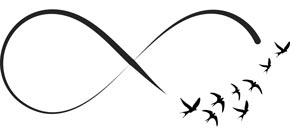
\includegraphics[width=0.44\textwidth]{./infinity.jpg}
  
  \vspace*{2\baselineskip}
  \textit{``fides in stellis, virtus in numeris"}
  
  \pagebreak
  
  \endgroup
}

\begin{document}

\title{\rmfamily\normalfont{Nexus: A Peer-to-Peer Network}}

\date{July 4, 2017}
    
\maketitle

\begin{abstract}

\noindent{\textit{``You never change things by fighting the existing reality. To change something, build a new model that makes the existing model obsolete"}}

\begin{center}
R. Buckminster Fuller
\end{center}
\bigskip

\noindent{Throughout history we have witnessed many changes in our culture, technology, and governance.}
These changes are fueled by a necessity for the further evolution of mankind.
Now humanity approaches another one of these times in history, where the way everything has been done must be changed; this is why we built Nexus.
Peer-to-Peer technology fuels the backbone of a global blockchain-based cryptocurrency represented by the ticker: \textit{NXS} which is traded world-wide as an alternative currency with the capacity to rival world economies.
The framework, Nexus, utilizes new distributed database designs, mathematical trust, community governance, ground-based mesh networks, and a \textit{Low Earth Orbit} Satellite Constellation.
We are Nexus, a connection of people, ideas, and computers providing greater choice and therefore greater evolution with an aim towards our freedom.
Welcome to the Future.
   
\end{abstract}

\newpage

\tableofcontents
\newpage
\maketitlepage
  {kSmith, pSmith, jSmith}


\paragraph{\textbf{\textit{Genesis} White Paper} - \textit{1.0.4} - Last Revised \today  }

\paragraph{}



\begin{wrapfigure}[4]{l}{0.40\textwidth}
    \centering
    \vspace{-25pt}
    \hspace{-15pt}
    
\includegraphics[width=0.30\textwidth]{./images/IMG_1228.JPG}
\end{wrapfigure}

\epigraph{nexus: a connection or series of connections linking two or more things.}{\textit{\footnotesize{Oxford English Dictionary}}}

\section{Introduction}

Peer-to-peer networks are forming the foundations of digital industries worldwide.
This ecosystem continues to evolve as innovators advance the growing body of open-source protocols, including \textit{Bitcoin, BitTorrent, TOR, and IPFS}.
The utility of these networks has increasingly affected people throughout the world.
For the first time in history, the transmission of value can occur without the need for intermediaries.
Now, almost ten years from the release of Satoshi Nakamoto's \textit{Bitcoin: A Peer-to-Peer Electronic Cash System} \cite{bitcoin} debuted on a Cypher Punk e-mail list in a time of economic crisis, many benefits have been realized including but not limited to: \textbf{\textit{viz.}} enhanced financial security, emancipation from centralized banking systems, and the possibilities of future applications of blockchains. However, many challenges have also been identified such as scaling, consensus updates, and considerations for the post-quantum era that is almost upon us.
By resolving some of these identified issues, Nexus has enhanced the blockchain protocol, thereby providing a solid foundation for the digital economies of the future. 
\bigskip

\subsection{What is Nexus?}
Nexus is a connection, or series of connections, of computers, businesses, and people with a focus on establishing new applications of finance, technology, service, and sovereignty.  

\subsection{What is a Blockchain?}

A blockchain is a decentralized and immutable public database of transactions. 
The database is organized by connecting a chain of blocks together.
Each block contains a group of transactions.
The blocks are ordered in time and linked together using cryptographic hashes.\footnote{"A cryptographic hash function is a hash function which takes an input (or 'message') and returns a fixed-size alphanumeric string. The string is called the 'hash value'..." \cite{wikihash}}\footnote{The concept of a cryptographic chain of blocks dates back to Ehrsam, Meyer, Smith and Tuchman's invention of Cipher Block Chaining (CBC) in 1976 \cite{cbc}. NB: this is distinct from \textit{blockchain} as discussed here in many ways, notably because it does not include a proof-of-work.}
Large quantities of computational resources must be expended to create each block hash,\footnote{This is generically called Proof-of-Work but also includes Sunny King's innovation: Proof-of-Stake \cite{peercoin}.} and each block contains the previous block's hash: \textit{this is how they are chained}.

\begin{center}
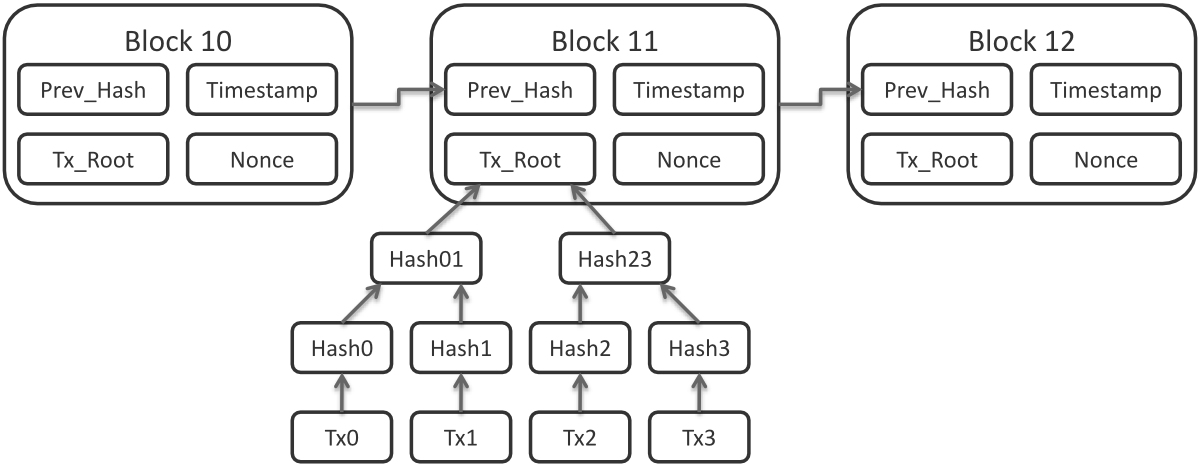
\includegraphics[width=0.80\textwidth]{./blockchain.png}
\end{center}
The blocks are produced in intervals, forming a chain of verifiable blocks that contain the transaction history providing data a form that cannot be altered without redoing the work of the \textit{previous blocks} or \textit{confirmations}.
The end result is a single, immutable journal of transactions grouped through time-ordered blocks distributed and verified by all of the nodes on the network.


\subsection{How are Blocks Created?}

Blocks are created by a distributed network of miners \textit{(users operating special hardware to solve the proof of work puzzles)} in a process called mining.
As an analogy for mining, imagine many people are sitting in a room out of motivation to win a prize if they solve their Rubik's Cube first.
The tiles of the Rubik's Cube can be thought of as the transactions, with one of these tiles representing the prize \textit{(mint)} the winner is allowed to claim if they solve the cube. 
However, they are only allowed to make one random change per iteration and they are limited by the speed of their hands \textit{(some may be faster than others)}.
Eventually one player will end up with a solved cube.
When one finds the solution, they show it to the other players in the room.
If the other players independently verify that the cube is solved properly, the winner is rewarded with the prize and a new round begins.

\subsection{Are Blockchains the Answer?}

Blockchains have become more necessary as we become aware of the challenges we are facing in our current progression as a society.
By maintaining open minds to recognize the challenges we face, we become aware of the limitations that legacy monetary systems cannot solve. 
As is seen that \textit{blockchains} do solve many monetary challenges, such as uncontrolled inflation, central banking, and many others, they are only a part of the solution to our current economic circumstances.

\epigraph{quantitative easing: unconventional monetary policy in which a central bank purchases government securities or other securities from the market in order to lower interest rates and increase the money supply}{\textit{Investopedia}}

\vspace{-138pt}
\hspace{-25pt}
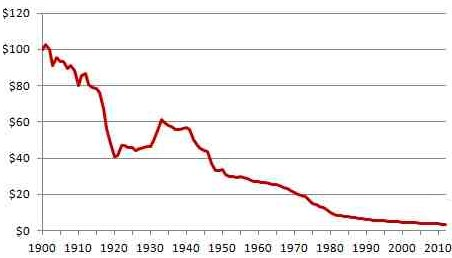
\includegraphics[width=0.60\textwidth]{./images/us-dollar.jpg}
\vspace{5pt}

\noindent
The term \textit{blockchain} should not be confused with any encrypted database. The dollar is essentially an online virtual currency encrypted between banks that is redeemable for federal reserve notes \textit{Paper Money}. This does not make the dollar a blockchain. What makes a blockchain is a decentralized public journal with no central authority. 
By owning a particular portion of a cryptocurrency, you prove partial ownership in the financial system.

\subsection{Challenges of Money}

The application and implementation of the world's monetary systems has become the source of one of the biggest challenges we face today.
This is due to the many global policies designed for empowering central banks to create currencies as debt with interest associated. 
Central Banks have the ability to influence world economies by changing interest rates, printing massive sums of money \textit{(otherwise known as inflation / hyperinflation)}, quantitative easing, or through various other forms of credit creation.
There are many historical examples of central authorities who have misused this enormous power, knowingly or unknowingly, to the detriment of the people that these institutions exist to serve. 
These include post-World War I Germany with a hyperinflation of up to 30,000\% per month, Zimbabwe during the Great Recession of the last decade with nearly 79 billion percent per month inflation, and post-World War II Hungary, with inflation rates of nearly \textit{13,000,000,000,000\%} per year.  \footnote{The estimated 200\% per day inflation equates to about thirteen quadrillion percent per year \cite{hyperinflation}}.


\section{Nexus}

Multiple components need to be considered when providing the fundamental basis for change and freedom.
The following is a brief outline of the core components that comprise the foundation of Nexus.

\subsection{Hardware}

Nexus is researching and developing three types of networks that will work together to form a new telecommunications system. 
These are outlined in the sections below.

\subsubsection{Mesh Networks}

\begin{wrapfigure}[14]{l}{0.44\textwidth}
    \centering
    \vspace{-20pt}
    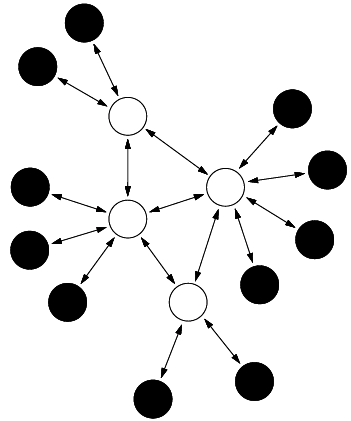
\includegraphics[width=0.44\textwidth]{mesh.png}
\end{wrapfigure}

A mesh network is a network topology in which each node relays data for the network. All mesh nodes cooperate in the distribution of data in the network \cite{meshnetworks}.\\ 

\noindent 
This allows for the growth of ground-based networks to handle data exchange in localized areas. \\

\noindent Ground-based mesh networks will solve many telecommunication issues.
Specialized antennas can be produced for people to purchase and operate, thereby forming networks owned by the individuals who built it.

\subsubsection{Cube Satellites}

As mesh networks grow, they will need to overcome the problem with line of sight and transcontinental communication. 
% * <maramichael@q.com> 2017-07-04T03:07:19.811Z:
% 
% > the problem
% What is the problem? The reader needs more detail so that they understand why this section is important to include.
% 
% ^ <maramichael@q.com> 2017-07-04T03:09:09.753Z.
This issue can be solved with the deployment of a satellite constellation designed to focus towards orbital cache layers and mesh network relays. 
This will provide caching of data and relaying of data between ground-based mesh networks.

\subsubsection{Ground Stations}

Ground stations will provide the satellite \textit{uplink/downlink} operations. 
These stations will be responsible for ground-based caching, the running of a nexus daemon, and the defining of a route to relay data to the addressed endpoint.

\subsection{Software}

There are many types of software applications that are integral parts of the functionality and efficiency of Nexus. The software systems are constantly being developed and improved upon as Nexus continues to mature.

\begin{itemize}
\item \textbf{Daemon}

Nexus operates on a lower-level software application called the \textit{"Nexus Daemon"}.
Instances of this software application communicate with one another, forming a peer-to-peer network.
They exchange data in the form of transactions and secure them into a distributed database called a blockchain.

\item \textbf{Wallet}

A command line and graphical Qt version of the Nexus wallet is currently available for download \cite{githubnexusreleases} \cite{nexusearth}.
A new version of the Nexus wallet will be a higher-level graphical application that allows access to the functions of the \textit{``Nexus Daemon"} through a HTML/JS interface. 
The interface also acts as a modular framework in which modules can be developed and sold for a greater user experience.\footnote{This is under active development at the time of this writing.}

\item \textbf{Library}

The lower-level library includes three parts, namely Crypto, Database, and Protocol. 
They form a lower-level set of programming base templates that can be used to create more complex class structures on top of them. 

\end{itemize}

\section{Specifications}

This section provides details on the specifications of the main software component of Nexus, the \textit{"Nexus Daemon"}.
This software component is the foundation of the Nexus Network and takes into account Precise Emission, Mining, Trust, and other components of security and efficiency. 

\subsection{Hashing}

Hashing is a critical part of any cryptocurrency.
The recent SHA-1 collision computation by Google underscores the need for more secure hashes \cite{googlesha1}. 
One of the innovations of Nexus is the use of newer hashing functions with the goal of enhanced security.

\subsubsection{SHA-2}

SHA-256 is a member of the SHA-2 set of cryptographic hash functions.\footnote{SHA stands for Secure Hashing Algorithm.}
It was designed by the National Security Agency (NSA) and published in 2001 \cite{wikisha2}.
SHA-256 is used in Bitcoin mining and in the creation of Bitcoin addresses \cite{bitwiki256}.

\subsubsection{SHA-3}

Nexus uses a newer, more secure hashing algorithm than that of Bitcoin.
The SHA-3 \cite{sha3} standard was the result of a competition \cite{nistcompetitionend} with the goal of producing an alternative to SHA-2.
This competition was organized by the National Institute of Standards and Technology (NIST).
The winner of this competition was selected in 2012.
The new SHA-3 standard algorithm is a subset of the cryptographic primitive family, Keccak \cite{nistgovk}.

\subsubsection{Skein}

The Skein algorithm was the runner up in the NIST hash function competition \cite{wikiskein}.
It is also used in Nexus, in combination with SHA-3.
The advantage of this approach is greater diversity in the secure hashing functions used in Nexus.

\begin{wrapfigure}{r}{0.50\textwidth} %this figure will be at the right
    \caption{Four of the 72 rounds of the Threefish-512 block cipher used in Skein \cite{skeinpaper}.}
    \centering
    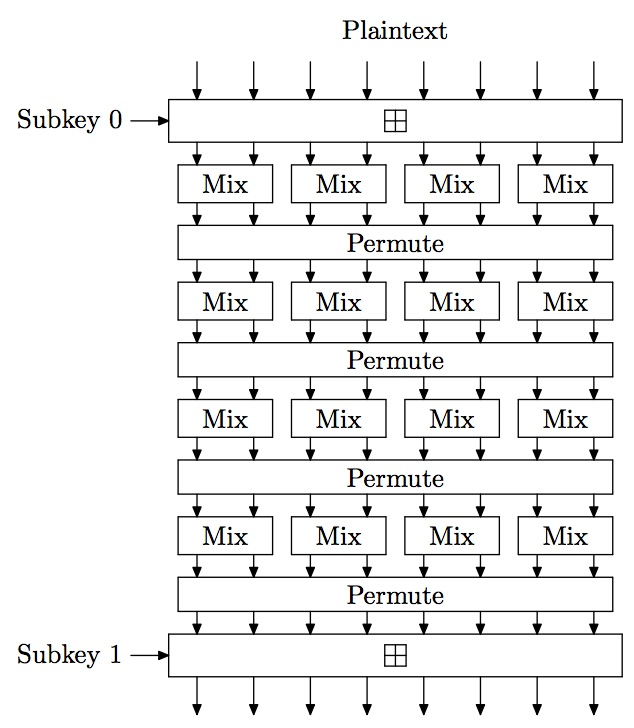
\includegraphics[width=0.50\textwidth]{skein-threefish-512-part.jpg}
\end{wrapfigure}

\pagebreak
\subsubsection{Skein-Keccak}

Nexus hashing is built from two secure hashing algorithms: Skein and Keccak \cite{sha3announce}. 
These two algorithms are combined to form a single SK-1024 (Skein-Keccak 1024 bit) hash. 
There are three types of output lengths in Nexus hashing: SK-256, SK-512, and SK-1024.
Public keys are hashed with SK-256 to secure them from public knowledge until spent. 
Transactions are hashed with SK-512 while SK-1024 is used for the proof-of-work hash.

%\epigraph{Moving forward, it's more urgent than ever for security practitioners to migrate to safer cryptographic hashes such as SHA-256 and SHA-3.\cite{googlesha1}}{\textit{\footnotesize{Google Research}}}

\subsubsection{Comparison of 256 bit and 1024 bit}

The following example illustrates the difference in size between a Nexus block hash and a Bitcoin block hash:

\begin{itemize}
\item Bitcoin Hash (256 bit)
\begin{lstlisting}
00000000000000000478710bb73175549d34893a375
454df1af122c26a453d9b
\end{lstlisting}

\item Nexus Hash (1024 bit)

\begin{lstlisting}
0000000001370e3764cffad92091c99b5beaf85f6fc
edae66e77be9de6f0ce6e3d8b1da4b6581d35f3ff6c
f359b10ab85c3b226f41cf864c979e8492f854c56d3
0e329ffc012c338caa7f3c6197137afb1637adc0b2f
22270990d0034c0ea0eae306ec28b7a565a1459896d
69a1c20f9f63af6c5fd672d76c6c8934e8363a21
\end{lstlisting}
\end{itemize}


\pagebreak
\subsection{Emission}

In Bitcoin, a fixed amount of BTC is available as a reward for miners in every block.
This amount halves every four years, thereby reducing Bitcoin's inflation.
However, this sudden change in the block reward is a shock to the market.
Miners spend large sums of money on equipment and personnel.
When the block reward halves, their profits are cut in half overnight.
\footnote{Theoretically because this reduction in profits can be foreseen, miners can prepare for it ahead of time.
Realistically, it's difficult for miners to account for this in a fast-changing system.}
Such uncertainty could possibly have a negative effect on network security \cite{cdhalving}.
\noindent Nexus improves upon this model by adjusting the reward with every block.
Using the equations for exponential decay \textit{(with carefully chosen constant $k$)}, ($e^{-kt}$), 
a deposit is made into reserves every minute.
The reserve determines the available reward for miners.\\ 

\noindent The supply is locked to time and not the block production rate. 
Inconsistent block times have no effect on the exact supply. 
This allows the projected supply to be accurately calculated at any second past the network time lock.

\subsubsection{Reserves}

A traditional water reservoir holds water that can be drawn upon by a town.
The total amount of water the town can draw is limited based on how much is in the reservoir.
In a similar way, the Nexus reserve system controls how much NXS is available to miners at a given time.\\ 

\noindent There are three reserves.
The amount of NXS deposited into each reserve is 
mathematically determined by the \textit{decay equations}.

\begin{equation}\label{eq:reserves}
\resizebox{.75\hsize}{!}{$
\begin{array}{ll}
      V_{d} = \;\;1 \cdot e^{-0.00000059 \cdot T_{m}} & + 0.032 \\
      V_{a} = 10 \cdot e^{-0.00000055 \cdot T_{m}} & + 1 \\
      V_{m} = 50 \cdot e^{-0.0000011 \cdot T_{m}} & + 1 \\
\end{array} $}
\end{equation}

\noindent Where $T_m$ is the time in minutes and $V_{d}$, $V_{a}$, $V_{m}$ are the reserve deposit amounts for miner, ambassador, and developer reserves.

\pagebreak
\subsubsection{Rewards}

The rewards are calculated based on the reserve value.
This prevents surplus emission beyond the target level.
\noindent These three equations describe the intervals in which the block reward $V_{b}$ changes
based on reserve values $V_{m}$ at $T_{m}$ by compounding the $T_{m}$ value from equations \ref{eq:reserves}.

\begin{equation}
\resizebox{.60\hsize}{!}{$
    V_b= 
\begin{cases}
    \frac{T_{a}}{60} \cdot V_{r}, & T_{m} \leq 2.5\\
    2.5 \cdot V_{r}, & 2.5 < T_{m} < 20\\
    3.0 \cdot V_{r}, & T_{m} \geq 20
\end{cases}
$}
\end{equation}

\begin{center}
Where $T_a$ is the actual time, $T_o$ is the offset time, and $T_t$ is the target time.\\
\end{center}


\subsubsection{Minting}

\begin{wrapfigure}{r}{0.50\textwidth}\label{fig:interestrate} %this figure will be at the right
    \centering
    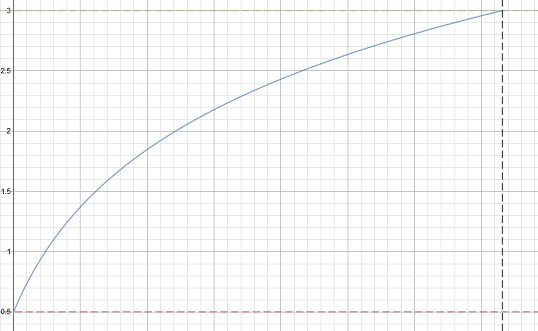
\includegraphics[width=0.50\textwidth]{interest.png}
    \caption{Interest Rate Graph.}
\end{wrapfigure}
%%Preston -Colin figure wrapping needs adjusted

Peer-to-peer networks, such as Bitcoin and Nexus, require the support of many nodes around the world.
If there aren't enough nodes, network stability, decentralization, speed, and security suffer.
Bitcoin suffers from a tragedy of the commons\footnote{The tragedy of the commons is an economic problem in which every individual tries to reap the greatest benefit from a given resource. As the demand for the resource overwhelms the supply, every individual who consumes an additional unit directly harms others who can no longer enjoy the benefits \cite{tragedycommons}.}
\noindent issue wherein everyone wants more people to run the peer-to-peer wallet, but there is little incentive to do so.
Nexus solves this problem by rewarding people with newly minted coins for holding Nexus and keeping their wallet up and running 24/7.
To put it simply, if someone installs the Nexus wallet on their computer and deposits enough NXS, then they will occasionally find a block and earn extra NXS.\footnote{This is a way to support the network and earn Nexus without costly and difficult-to-operate mining hardware and software.}\\

\noindent This minting system operates to give people larger rewards for greater contribution to the network. 
As one produces blocks by using this method in a timely manner, one's trust grows.
With a higher trust score comes a higher minting rate.
The minting rate $R_m$ ranges from 0.5 \% - 3 \%.

\paragraph{}
\begin{equation}
\resizebox{.65\hsize}{!}{$R_m = \frac{0.025 \cdot ln(\frac{9 \cdot a_{t}}{31449600} + 1)}{ln(10)} + 0.005$}
\end{equation}

\noindent Where $a_t$ is the age of your trust key (the number seconds since the trust key's genesis transaction).

\subsection{Block Validation}

There are three ways to produce a valid Nexus block and mint new NXS.
There are two proof-of-work channels and one proof-of-holdings channel.
The proof-of-work channels are the Prime Channel and the Hashing Channel.
In the Prime Channel, miners search for Dense Prime Clusters of ~308 digits in size.
In the hash channel, standard Hashcash \cite{hashcash} style work is computed using the SK-1024 hashing algorithm. 
The two proof-of-work channels prevent each other from producing too many blocks in a row, thus forcing a 51\% attacker across both channels.\footnote{Reserves between Prime and Hash are split evenly at 50 \%}

\subsubsection{Dense Prime Clusters}

The work done by miners in the Prime channel is a search for dense prime clusters \cite{wikiprimecluster}.\footnote{The numbers found in these searches are actually probable primes \cite{wikiprobable}. They pass the Fermat Prime test \cite{wikifermat} at base 2, 3, and 5.}
Finding these dense prime clusters is a trial-and-error process.
Miners must try many numbers to successfully find one that is the beginning of a dense prime cluster \cite{wolframprimecluster,primesolominer}.\\ 

\noindent The count of prime numbers in a dense prime cluster is called its chain length.
\footnote{The ``chain" here should not be confused with the chain in blockchain.}
A dense prime cluster with a longer chain length is more difficult to find than one with a shorter chain length.
The first prime number in the chain is required to be higher than the block hash and less than the block hash plus $2^{64}$.\footnote{The block hash can't be determined a priori for future blocks because it's based on previous block information. 
Therefore, a miner must start their prime cluster search over again after each new block is found.}
If the first prime in the cluster fits these criteria, it is considered a valid solution.\\

\noindent One benefit to searching for dense prime clusters is that it is thought to be more resistant to GPU, FPGA, and ASIC mining than hashing.
Another is that the data produced by the miner is useful for mathematical research into prime numbers \cite{findingprimeclusterspaper} \cite{nxsprimecom}.
The applications of prime number research may extend beyond mathematics and into quantum physics \cite{physicsmathprime}.
This is one of the ways that Nexus provides value back to the scientific community and the world.

\subsubsection{Hashing}

The hashing channel uses a \textit{Hashcash} \cite{hashcash} style proof-of-work.
Miners run code \cite{skminer,wolfniro} on GPU's in an attempt to find a hash that meets a given difficulty.
If they are lucky, they will find a hash with at least a certain number of leading 0 bits. 
This means that the hash is preceded by a number of 0's and is a smaller integer. 
This is called a "partial collision".
This is similar to the proof-of-work scheme that Bitcoin uses.
Bitcoin uses SHA-256 while Nexus uses the newer SHA-3 in combination with Skein.

\subsubsection{Holdings}

Proof-of-Holdings \textit{(POH)} provides a third channel of security.
An attacker would need to gain 51 percent of the NXS supply to attack this channel in conjunction with the hash and prime channels.
The incentive for this proof system is newly minted coins which are rewarded to participants for actively ``holding" their coins. 
This means the network incentives users to contribute to the security of the system. 
This provides a natural growth in the coin supply over time that will be highly beneficial to the network, economy, and users.\\ 

\noindent Unlike current Central Bank models, this new supply of coins goes directly into the users hands rather than being filtered through a fractional reserve system. 
Furthermore, these newly minted coins have zero debt associated with their issuance and, therefore, never need to be paid back to the system with associated interest, as is the case with many current fiat currencies.
The minting rate was determined to be a variable rate between .5\% and 3\% to provide a small natural growth to the coin supply allowing for increased economic opportunity.

\subsection{Difficulty}

The difficulty of finding a block is adjusted with every new block.
The Nexus difficulty algorithm combines weighted averages for the last $n$ blocks.
A weighted average time, $T_a$ is calculated as follows:\\ 

\begin{equation}
\resizebox{.75\hsize}{!}{$T_{a} = \frac{\sum_{i=1}^{n} w \cdot i [ T_b(H - n + i) - T_b(H-n+i-1) }{n}$}
\end{equation}\\ 

\noindent Where $H$ is the current block height, $T_b$ is the block time stamp at a given height, $n$ is the blockchain depth, and $w$ is a weight constant (currently set to 3).\\  

\noindent $Mod_d$ is the factor used to modify the difficulty\\ 

\begin{equation}
\resizebox{.70\hsize}{!}{$
    Mod_d= 
\begin{cases}
    [1 - (Min_{d} \cdot T_{o})] \cdot T_{t}, & \text{if } T_{a} \geq T_{t}\\
    [1 + (Max_{d} \cdot T_{o})] \cdot T_{t}, & \text{otherwise}
\end{cases}
$}
\end{equation}

\noindent Where $T_t$ is the target time, $T_o$ is the offset time, $Min_d$ is the minimum difficulty decrease and $Max_d$ is the maximum difficulty increase.

\epigraph{It's a vice to trust everyone, and equally a vice to trust no one.}{\textit{\footnotesize{Seneca}}}

\pagebreak
\subsection{Trust}\label{subsection:Trust}

Trust is a core component of Nexus.
Nodes which have a vested interest in and are acting to benefit the whole network by participating honestly and consistently are considered more trustworthy.
Currently, trust is earned by holding Nexus in a wallet and producing valid blocks on a regular basis.
This earned trust is recorded in the Nexus blockchain and is associated with a trust key.\\ 

\noindent Future areas of research and development in Nexus are focusing on using the concept of trust in many ways.
Using trust, a new security model can be developed around time.
The strength of the Nexus economy and its reliability will be reinforced by promoting truthfulness between the voluntary interactions with individuals and groups of individuals.

\subsubsection{Weight}

Weight governs the speed in which one can search for new trust blocks. 
It comes in the form of two different weight variables: Block Weight ($W_b$) and Trust Weight ($W_t$).

\begin{equation}
W_{t} = Min(17.5, \frac{16.5 \cdot ln(\frac{2 \cdot a_t}{2419200}) + 1}{ln(3)} + 1.0)
\end{equation}

\begin{equation}
W_{b} = Min(20.0,\frac{19.0 \cdot ln(\frac{2 \cdot a_b}{86400}) + 1}{ln(3)} + 0.05)
\end{equation}

\noindent Where $a_t$ is the trust age and $a_b$ is the block age.

\subsubsection{Threshold}

A system has been developed to allow an energy-efficient time-based trust system.
This is regulated by the Energy Efficiency Threshold $E_t$.

\begin{equation}
\resizebox{.22\hsize}{!}{$E_{t} = \frac{100 \cdot T_{a}}{N_{once}}$}
\end{equation}

\pagebreak
The Required Threshold $R_t$ is

\begin{equation}
\resizebox{.5\hsize}{!}{$R_{t} = \frac{(50 - W_{t} - W_{b}) \cdot 1000}{C}$}
\end{equation}

Where C is the total NXS in a trust transaction.

\subsubsection{Genesis}

The genesis transaction is the first transaction of a trust key. 
This is required to act as the root of the trust key's age in order to gain a reference on its current weight and minting rate. 
The hash of this genesis transaction can therefore be used as an input in future transactions to verify that a trust block is linked to a corresponding genesis transaction.

\noindent The following equation describes the genesis weight required to get a high enough threshold to achieve the creation of a genesis transaction and corresponding block\footnote{Genesis transaction weight does not include block weight.}

\begin{equation}
\resizebox{.70\hsize}{!}{$
W_{g} = Min(17.5, \frac{16.5 \cdot ln(\frac{2 \cdot a_{c}}{7257600}) + 1}{ln(3)} + 1.0)
$}
\end{equation}

\noindent Where $a_c$ is the coin age of the coins which are being used.

\subsubsection{Intervals}
 
Trust blocks cannot be created from the same trust key unless the interval or number of blocks between their last trust block exceeds $I_{t} \geq 6$.

\subsection{Clock Drift}

Clock drift refers to several related phenomena where a clock does not run at exactly the same rate as a reference clock \cite{wikiclockdrift}.
This is usually resolved by connecting to a central server and/or atomic clock.
Nexus combats this with a peer-to-peer time-keeping system that keeps all clocks on the network synchronized to the unified time seed.

\subsection{Security}

Bitcoin and other cryptocurrencies allow up to 2 hours in the future for clock drift, which means that blocks can be created up to 2 hours from the current network \textit{timestamp}, thereby leaving potential attack vectors.
Nexus combats this synchronization not with median time, as Bitcoin uses, but rather with a Unified Time system that operates on the protocol level keeping all Nexus clocks synchronized to the second.

\subsection{Time-Locks}

Because clocks in the Nexus network are synchronized, new rules can be activated in the protocol based on time stamps rather than block numbers.
This allows network participants to more accurately activate consensus updates.

\subsection{Checkpoints}

Automated decentralized checkpoints are created every hour.
A checkpoint prevents any block that was not rooted from the last hardened checkpoint to be invalid.
This prevents an attacker from producing an alternative blockchain prior to the last checkpoint time.

\bigskip
\epigraph{I think I can safely say that nobody understands quantum mechanics.}{\textit{\footnotesize{Professor Richard Feynman, 1965 Physics Nobel Laureate \cite{nobelfeynman}}}}

\pagebreak
\section{Post-Quantum Considerations}

\begin{wrapfigure}{r}{0.60\textwidth} %this figure will be at the right
	\vspace{-35pt}
    \centering
    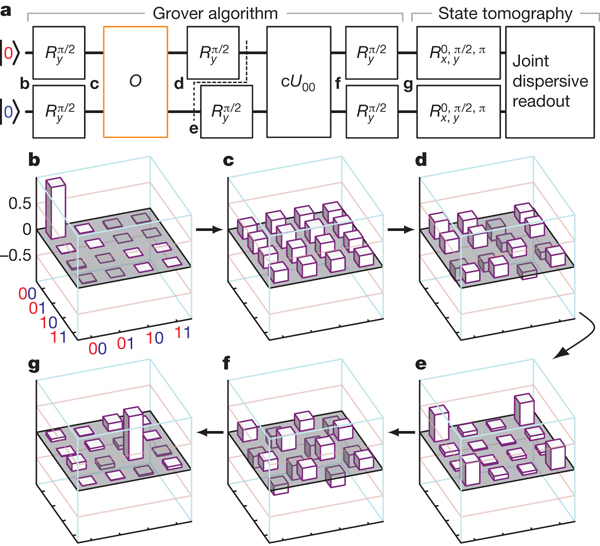
\includegraphics[width=0.50\textwidth]{grovers.jpg}
    \caption{Grover's Algorithm on Two Qubits}
\end{wrapfigure}

\subsection{Grover's Algorithm}

Grover's algorithm is a quantum algorithm which was devised by Lov Grover at Bell Labs.
The summary in Grover's 1996 paper provides a helpful description:
"Imagine a phone directory containing N names arranged in completely random order. 
In order to find someone's phone number with a probability of one half, 
any classical algorithm... will need to look at a minimum of $N/2$ names. 
Qubits can be in a superposition of states, which means that a qubit can be either a 0 or a 1.
As a result, the desired phone number can be obtained in only $O(\sqrt{N})$ steps \cite{lovgrover}."\\ 

\noindent Given the output of a black box function, it can be used to determine\footnote{In a probabilistic manner.} the input.
This implies that most one-way cryptographic hash functions are susceptible to this algorithm.
Indeed, Grover's algorithm could brute-force a 256-bit key in roughly $2^{128}$ iterations.\\ 

\noindent The algorithm proceeds to call $G$ $[\frac{\pi}{4} \cdot 2^{\frac{k}{2}}]$ times in the verification of the subroutines. The largest overhead, though, in Grover's Algorithm is the cost of error detection that must be done classically to ensure the accuracy of the qubits (overcoming quantum noise), and the two subroutines of Grover Iteration.\\


\begin{table}[ht]
\caption{Resource Comparison for Grover Search of SHA-256 and SHA3-256 \cite[p.~18]{groversalgorithm}}
\begin{center}
\begin{tabular}{c|ccc|}
    \hline
    \hline
    & & \textbf{SHA-256} & \textbf{SHA3-256} \\
    \hline
    \multirow{4}{*}{\rotatebox[origin=c]{90}{Grover}}
    &T-count & $1.27 \cdot 10^{44}$ & $2.71 \cdot 10^{44}$ \\
    &T-depth & $3.76 \cdot 10^{43}$ & $2.31 \cdot 10^{41}$ \\
    &Logical qubits & $2402$ & $3200$ \\ 
    &Physical qubits & $1.39 \cdot 10^{7}$ & $1.94 \cdot
    10^{7}$ \\
    \hline
    
    \multirow{4}{*}{\rotatebox[origin=c]{90}{Distilleries}}
    &Qubits per Distillery & $3600$ & $3600$ \\
    &Total Distilleries & $1$ & $294$ \\
    &Code Distilleries & $\{33, 13, 7\}$ & $\{33, 13, 7\}$ \\ 
    &Physical qubits & $5.54 \cdot 10^{5}$ & $1.63 \cdot
    10^{8}$ \\    
    \hline
    
    \multirow{4}{*}{\rotatebox[origin=c]{90}{Total}}
    &Logical qubits & $2^{12.6}$ & $2^{20}$ \\ 
    &Code Cycles & $2^{153.8}$ & $2^{146.5}$ \\
    &Total Cost  & $2^{166.4}$ & $2^{166.5}$ \\
    
    \hline
    \hline
\end{tabular}
\end{center}
\end{table}
%bdg% Table reviewed, matches info from referenced paper, page 18.

\noindent The first subroutine of $G$ is attempting to assert g : $\{0, 1\}^k \rightarrow \{1, 0\}$ maps $X$ to $1$ only if $f(x) = y$. 
The next subroutine is called the \textit{``Diffusion Operator"}, and it implements the transformation of g to increase the probability that $f(x) = y$.\\ 

\noindent As illustrated in Table 1, Grover's Algorithm results in a nearly 50\% reduction to the security provided by one-way hashing functions against brute-force attacks.
This implies that a hash, which has twice as many bits, should be used to achieve the same level of security against brute-force attacks.


\subsection{Elliptic Curve Cryptography}

Elliptic Curve Cryptography, in terms of classical computing, retains high security standards with smaller key sizes compared to RSA \cite{wikikeysize}.
The following equation can be used to represent an elliptic curve:

\begin{equation}
\resizebox{.33\hsize}{!}{$y^2 = x^3 + ax + b$}
\end{equation}

%%Preston -Colin figure wrapping needs adjusted

\subsection{Curve Groups and Fields}


\begin{wrapfigure}[8]{r}{0.40\textwidth} %this figure will be at the right
\vspace{-40pt}
\caption{Illustration of an Elliptic Curve}
    \centering
    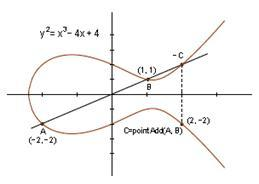
\includegraphics[width=0.40\textwidth]{ecc.JPG}
\end{wrapfigure}

In Nexus, the elliptic curve domain parameters are based on \textit{sect571r1} \cite{sect571r1} as defined in the ``Standards for Efficient Cryptography 2: Recommended Elliptic Curve Domain Parameters" and they are defined over a binary field $\mathbb{F}_{2^m}$.
The domain parameters that are used in most other digital currencies are based on \textit{secp256k1} \cite{secp256k1}. These parameters are associated with a Kolbitz curve and are defined over a prime field  $\mathbb{F}_p$.

\subsection{Private Keys}

A private key is a number that should only be known to the owner of the coins in a given address.
To produce a secure private key, it's necessary to start with a number that is as close to truly random as possible.\footnote{This is handled by the Nexus wallet software - it generates private keys and stores them.}
If anyone is able to determine what the private key is, they can move the coins to another address.
This is why private key security is so important.
You don't want anyone else to find out what your 'secret number' is, 
and you don't want them to be able to guess it or determine it with a complex algorithm based on public information.
Both Bitcoin and Nexus use large numbers so that there is almost no chance that anyone else will generate the same random number, and it is impossible for anyone to try all of the numbers.\footnote{"How many numbers? For every grain of sand on Earth, create a new Earth. There are 26 billion unique Bitcoin addresses for each grain of sand on each of those Earths."\cite{weusesand} Because the keys in Nexus are longer, there are astronomically more possible Nexus addresses.}
Bitcoin keys are 256 bits in length, while Nexus keys are more than twice as long at 571 bits.

\bigskip
\textbf{Bitcoin Private Key (256 bit)}
\begin{lstlisting}
5Kb8kLf9zgWQnogidDA76MzPL6TsZZY36hWXMssSzNydYXYB9KF
\end{lstlisting}

\bigskip
\textbf{Nexus Private Key (571 bit)}
\begin{lstlisting}
6Wuiv513R18o5cRpwNSCfT7xs9tniHHN5Lb3AMs58vkVxsQdL4atHTF
Vt5TNT9himnCMmnbjbCPxgxhSTDE5iAzCZ3LhJFm7L9rCFroYoqz
\end{lstlisting}

\subsection{Public Keys}

It's easy to derive a public key from a private key, but not a private key from a public key.
When you request a payment from someone, you first get a \textit{Nexus address} from your wallet.
This address is not your public key, it is called a public key hash, or \textit{PKH}.
As the name implies, it's created by hashing your public key and converting it into Base58 encoding.
This means that an attacker who wants to figure out your private key first has to determine your public key from the \textit{PKH}.
Fortunately, this is an intractable problem. Current research indicates this may take even quantum computers on the order of a hundred billion years \cite{registersha3,cryptosha3} to reveal the public key.
The public key associated with a \textit{PKH} is not revealed until the coins are spent \cite{bitcorepkh}.
Therefore, one can achieve a high level of quantum attack resistance simply by not re-using addresses.\\

\subsection{Shor's Algorithm}

\noindent In 1994, Peter Shor created an algorithm which could be used to solve the Integer Factorization Problem \textit{IFP} and the Discrete Logarithm Problem \textit{DLP} in polynomial time on a quantum computer \cite{shorarxiv}.
This was an important achievement because these problems have no classical polynomial time solution.
This means that, on a classical computer, they can't be solved in any amount of time which can be represented by $n^k$ - for example $n^2$, $n^3$, etc.\footnote{In layman's terms, this means that finding a solution is infeasible as long as a large enough number is used.}\\ 

\noindent The Elliptic Curve Discrete Logarithm Problem \textit{(ECDLP)} is a special case of the \textit{DLP} for elliptic curves.
This is a more difficult problem to solve classically than conventional cryptography relying on the \textit{DLP} alone.\cite{prooszalka} % Section 2.1.2
This is the type of problem that needs to be solved in order to determine the private key from the public key for cryptocurrencies, such as Bitcoin and Nexus.\\

\subsection{Proos-Zalka Algorithm}

The Proos-Zalka algorithm was specifically designed to solve the \textit{ECDLP} over a prime field $\mathbb{F}_p$ on a quantum computer.
The qubit requirement for the breaking of the ECDLP over a prime field of $n$ bits is as follows \cite{prooszalka}

\begin{equation}
\resizebox{.5\hsize}{!}{$5\cdot n + 8 \sqrt{n} + 4 \log_{2} n + 10 \approx 6n$}
\end{equation}

\subsection{Kaye-Zalka Algorithm}
The Kaye-Zalka revision addresses curves over the binary field $\mathbb{F}_{2^m}$. This specific field takes advantage of binary computation to bring quicker verification on larger keys. The equation modeling the qubits required to break a key of $\mathbb{F}_{2^m}$ is as follows \cite{kayezalka}.

\begin{equation}
\resizebox{.5\hsize}{!}{$2 m + 7\cdot log m + 7 + H \approx 2m$}
\end{equation}

\noindent Where H is related to the halting counter and is of order $log(m)$.

\subsection{The Benefits of Larger Keys}

"Key length defines the upper-bound on an algorithm's security since the security of all algorithms can be violated by brute force attacks \cite{wikikeysize}." \\ 

\noindent As of 2015, a minimum key length of 224 bits is recommended for elliptic curve algorithms \cite{bruteforce}.
Bitcoin keys are $256-224 = 32$ bits longer than this requirement while Nexus keys are $571-224 = 347$ bits longer.
\noindent According to the National Security Agency 
``Elliptic Curve Public Key Cryptography using the 256-bit prime modulus elliptic curve as specified in FIPS-186-2 and SHA-256 are appropriate for protecting classified information up to the ``secret'' level. 
Use of the 384-bit prime modulus elliptic curve and SHA-384 are necessary for the protection of ``top secret'' information \cite{nsa384}."

\subsubsection*{Brute Force Resistance}

The Large Bitcoin Collider \cite{largebitcoin} is a project that attempts to brute force-attack Bitcoin.
Participants in this project generate as many Bitcoin public addresses as possible by first choosing a random number in a given range.
Rarely do they find a public address that contains Bitcoin, but on chance one is discovered the Bitcoin contained in it can be stolen.\footnote{There are a couple of ways to mitigate the risk of such an attack on your Bitcoins. First, don't keep too many coins in one address. Second, use multisig.}\\

\noindent Key length defines the upper-bound on an algorithm's security \cite{wikikeysize} against brute-force attacks.
Nexus uses significantly larger 571-bit keys than Bitcoin's 256-bit keys and is thus postulated to be more resistant to these attacks.\\ 

\noindent In any case, Rico - the pseudonymous lead of the LBC states: "Finding a P2PKH\footnote{Pay to Public Key Hash\cite{p2pkh}}-collision [one cryptographic method of creating Bitcoin addresses] would probably mean the end of P2PKH but not Bitcoin," ... "Bitcoin would evolve with new address types. Most certainly it wouldn't 'die' because of this."\cite{largebitcoin}
This highlights one of the ways that Nexus is providing value back to the Bitcoin ecosystem.
By using different elliptic curve parameters and different hashing algorithms, Nexus is paving the way for possible future enhancements to Bitcoin.
Instead of merely researching or discussing alternatives, Nexus has been proving them on a live blockchain.

\subsubsection*{Longer Solution Time}

It will take more time for a quantum computer to solve the \textit{ECDLP} if the key is larger.
The run times are predicted to be of order $O(n^2)$ to $O(n^3)$ \cite{prooszalka,kayezalka}.
This means that a key which is twice as long will take approximately four times as long to find with a quantum computer.

\begin{table}[ht]
\caption{Qubits and Time required to break each key size for $\mathbb{F}_{p}$ \cite{quantumattacks}}
\begin{center}
\begin{tabular}{|c|c|c||c|c|c||c|}
    \hline
    \multicolumn{3}{|c||}{Quantum IFP} &
    \multicolumn{3}{c||}{Quantum ECDLP} &
    Classical \\
    \hline
    $\lambda$ & Qubits $\lambda$ & Time $4 \cdot \lambda ^ 3$ & $\lambda$ & Qubits $7 \cdot \lambda$ & Time $360 \cdot \lambda ^ 3$ & Time \\
    \hline
    \hline
    512 & 1024 & $0.54 \cdot 10^9$ & 
    110 & 700  & $0.50 \cdot 10^9$ & $c$ \\
    
    1024 & 2048 & $4.30 \cdot 10^9$ & 
    163  & 1141 & $1.60 \cdot 10^9$ & $c \cdot 10^8$ \\
    
    2048 & 4096 & $34 \cdot 10^9$ & 
    224  & 1568 & $4.0 \cdot 10^9$ & $c \cdot 10^{17}$ \\
    
    3072 & 6144 & $120 \cdot 10^9$ & 
    256 & 1792  & $6.0 \cdot 10^9$ & $c \cdot 10^{22}$ \\
    
    15360 & 30720 & $1.5 \cdot 10^{13}$ & 
    512   & 3584  & $50 \cdot 10^9$ & $c \cdot 10^{60}$ \\
    \hline
\end{tabular}
Where $\lambda$ is the input length in bits.
\end{center}
\end{table}

\subsection{Side Channel Attacks on secp256k1}

As previously mentioned, Bitcoin uses the 256 bit \textit{secp256k1} elliptic curve domain parameters as defined in the Standards for Efficient Cryptography.
Under special circumstances, a Bitcoin private key can be determined by another process on the same classical computer in as few as 200 signatures \cite{sigleak}.\footnote{This is called a "side channel" attack.}
With quantum computing on the horizon, and the fact that ECC already leaks private keys classically with side channel attacks, serious considerations must be made on the logic of any use of digital signature algorithms to prove ownership of any tokens.
This is the focus of ongoing research and development in Nexus.

\subsection{Key Accommodations in Nexus} 

Nexus currently supports key sizes as large as 571 bits, specifically sect571r1.
In order to offer more choice and to take advantage of the larger number of qubits required to crack curves over prime fields, we will also implement keys using different curves.\\

\noindent The choice of elliptic curve parameters is subtle; care must be taken to avoid security pitfalls.
We plan to add support for multiple curves including post quantum solutions being developed at the current time.
To mitigate against quantum attack, signature chains will be included as a part of the Tritium protocol taking advantage of \textit{PKH} and \textit{OTS} or one-time signatures, which happen to prevent side channel attacks and make quantum attacks exclusive to Grover's Algorithm.
The projected time before quantum computers reach dangerous levels is the around five to ten years.
By doubling Nexus key sizes, the required run time is quadrupled; this provides more time to carefully choose a post quantum cryptographic method. 
This is projected to be within the next few years as the development of post-quantum cryptography is observed and studied more thoroughly.

\subsection{Post-Quantum Cryptography}

There are many promising solutions to the post-quantum conundrum that we are facing in the coming years. 
One of which holds promise is lattice based cryptography which ensures that quantum attack, at least for now, is infeasible. 
Another viable solution to such attacks is using hash based signatures such as \textit{XMSS} which does hold certain characteristics of post-quantum solutions, but it does carry a heavy drawback of requiring very large amounts of data to be transfered in order to protect the private key from being leaked. 
This is not desirable when selecting a DSA \textit{Digital Signature Algorithm} for a blockchain, as there are already very high data overheads that haven't been addressed in scaling solutions.
NIST just opened a new competition for Post-Quantum standardization similar to the SHA3 competition that should be finalized in the next few years to give us a better selection of post quantum algorithms. \cite{NIST_POST_QUANTUM} 

\section{Conclusion}

With modern hashing, upgraded private keys, multiple block validation methods, decentralized checkpoints, time synchronization, decentralized trust, variable block reward, time locked emission, decentralized minting, lower level library, quantum considerations, ground based mesh networks, and low earth orbit satellite constellation; Nexus is one of the most technologically advanced frameworks on the planet. 
We now have an opportunity to step away from existing systems by simply changing our focus. 
We can choose to look away from the systems of the past and focus our thoughts on the systems of the future. 
Nexus exists as a publicly available, free-to-use, peer-to-peer network for people to connect and improve the quality of their lives.  
Peer-to-Peer technologies have the capability to help us reshape our world and Nexus represents an important step forward in this process. 
The noun ``nexus'' is defined as: a connection or series of connections linking two or more things. 
Nexus is an idea of connection and the technology to make this possible.
It is through this connection that we can create a future filled with life, liberty and the pursuit of happiness.
Welcome to Nexus.
\pagebreak

\appendix

\section{Appendix: Reference Summaries to Reinforce Content}

This appendix is designed to be seen ``as an extension to the core content'' as references to the ideas described herein.
With the understanding and study of the following sections, one can gain a higher level perspective of what needs to be understood for us to progress as a species.
As we can see, societal organization models, ancient philosophies that have stood the test of time, and preliminary principles designed to be references to greater understanding of truth are described below.

\epigraph{Action without Vision is a Daydream, Vision without Action is a Nightmare.}

\section{Vision}

Vision is one's ability to think about or plan the future with wisdom.
Wisdom is the quality of having experience, knowledge, and good judgment. 
In this case, vision is coupled with wisdom, which is a direct result of experience and, therefore, knowledge. 
This means that vision is attainable if one is willing to learn from the experience of the world.
Vision can be understood at a greater depth by applying the following to conduct:
\begin{enumerate}
\item \textbf{Capable} of verifying and/or understanding without premature conclusion
\item \textbf{Discipline} to see \textit{what is} - unaltered by definitions and belief systems
\item \textbf{Knowledge} gained through the study of reality, society, and the work of others
\item \textbf{Accordance} with the laws of nature, virtue in accordance with the laws of the self
\item \textbf{Principle} formed through the understanding of this accordance
\end{enumerate}

\section{Philosophy}

Philosophy is the study of the fundamental nature of knowledge, reality, and existence - \textit{as it is} - with intent to understand \textit{what it is}. 
Following will include a short list of philosophies forming a foundation for vision and principle to integrate into greater virtue, reason, and success in the form of happiness being the ultimate value in which each individual seeks.

\begin{center}
\textit{
I must not fear.\linebreak
Fear is the mind-killer.\linebreak
Fear is the little-death that brings total obliteration.\linebreak
I will face my fear.\linebreak
I will permit it to pass over me and through me.\linebreak
And when it has gone past I will turn the inner eye to see its path.\linebreak
Where the fear has gone there will be nothing. \linebreak
Only I will remain.\linebreak
}
\footnote{Bene Gesserit Litany Against Fear - From Frank Herbert's Dune Book Series}
\end{center}

\begin{wrapfigure}[17]{r}{0.44\textwidth}
    \centering
    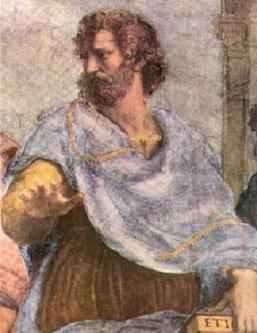
\includegraphics[width=0.44\textwidth]{aristotle.jpg}
\end{wrapfigure}

\subsection{Nicomachean Ethics}

Aristotle was an ancient Greek philosopher and scientist \cite{aristotle}. 
Aristotle believed that virtue was essential in achieving the ultimate goal: happiness.\\ 
\noindent As a portion of the philosophies described in his works on Nicomachean Ethics, an idea was formed under the name the \textit{"golden mean"} which described a world of excess and deficiency.
This philosophy described the evils of the world - or oppositions to the growth of life - to be either excess or deficiency. 
The golden mean is described as the quality of having neither excess or deficiency but rather a "golden mean" between the two extremes. 

\pagebreak
\subsection{Kingdom of Ends}

\begin{wrapfigure}{l}{0.44\textwidth}
    \centering
    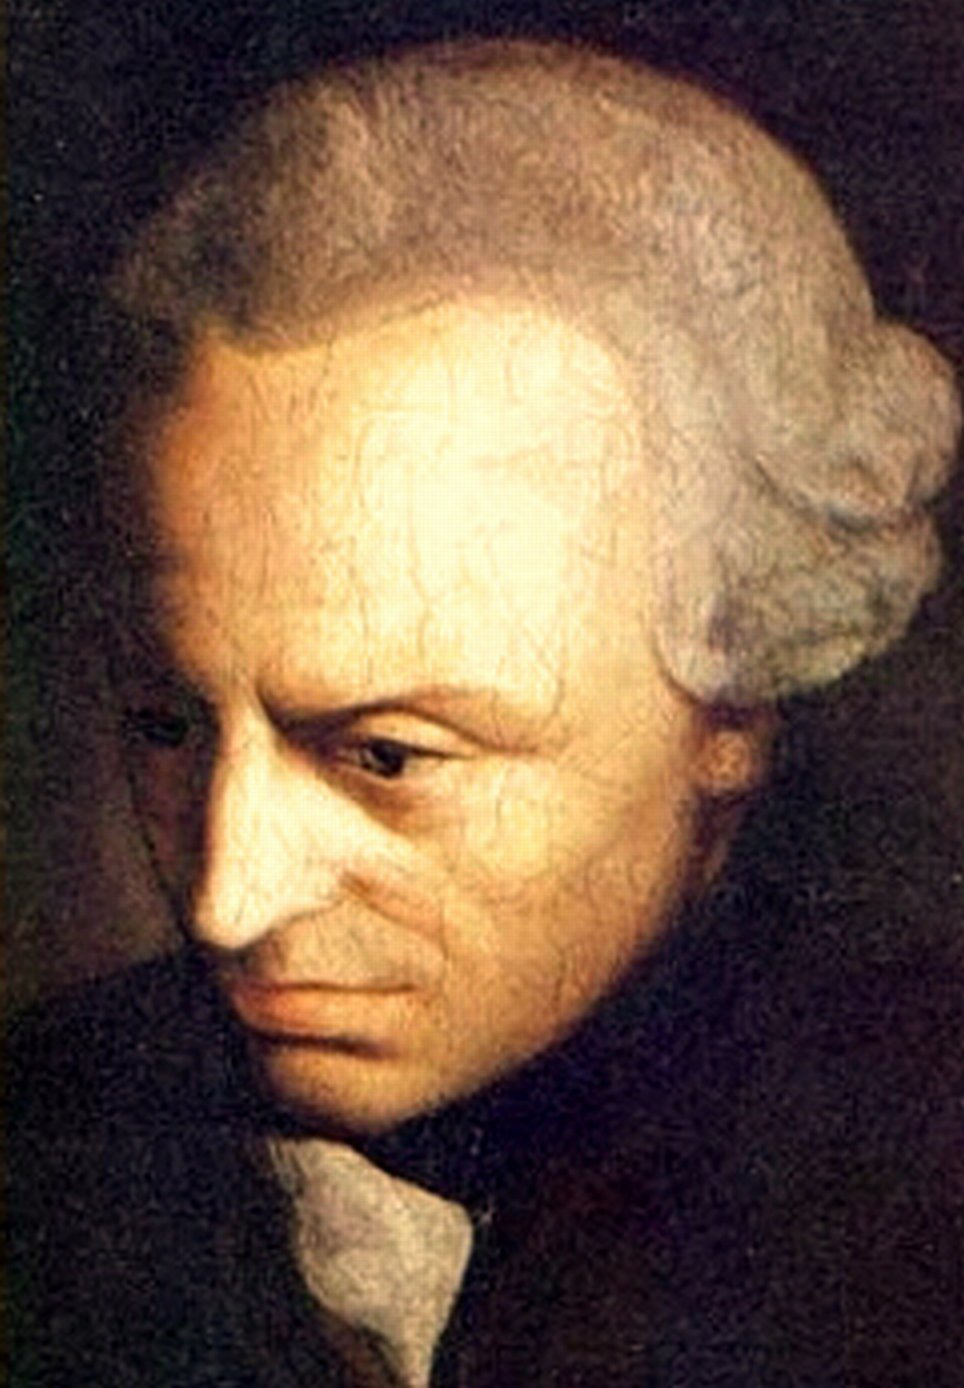
\includegraphics[width=0.44\textwidth]{kant.jpg}
\end{wrapfigure}

Immanuel Kant was born ahead of his time on the 22nd of April, 1724 in Berlin, Germany \cite{kant}. He had many philosophies that are still studied to this day. 
One of his more notable works was called the \textit{Kingdom of Ends}. 
He describes a hypothetical existence where individuals act entirely rationally, and with reason.
He defines these people as ones capable of proper conduct. 
He proposed that when those that were capable were able to live under a common law of laws that were of the utmost importance and necessity, that a more harmonious and \textit{moral} society could form as a \textit{Kingdom of Ends}.\\

\noindent These common laws could be considered reference points for the value of actions in a Kingdom of Ends, to where its correlation with universal law provides the greatest value to those of the Kingdom of Ends.
His second formulation showed that individuals that live in accordance with the principle to treat ones fellowmen as end in themselves, were capable of greater virtue, and therefore, joy.
This describes an idea and philosophy of acting in accordance and harmony with one's people as a kingdom of ends, rather than each individual seeking one another as means to their own ends.

\bigskip
\textit{"People can only belong to the Kingdom of Ends when they become subject to these universal laws. 
Such rational beings must regard themselves simultaneously as sovereign when making laws, and as subject when obeying them. 
Morality, therefore, is acting out of reverence for all universal laws which make the Kingdom of Ends possible. 
In a true Kingdom of Ends, acting virtuously will be rewarded with happiness."} \footnote{Excerpt quoted from \url{https://en.wikipedia.org/wiki/Kingdom_of_Ends}}

\subsection{The Tao}

In ancient China, the keeper of the Imperial Library, Lao Tzu, was famous for his wisdom. Perceiving the growing corruption of the government, he left for the countryside. On his way, the guard at the city gates asked Lao Tzu to write out the essence of his understanding to benefit future generations. Lao Tzu wrote the Tao Te Ching, left, and was never heard of again \cite{tao_introduction}.

\medskip
\begin{center}
\textbf{\cite{tao_chapter1} Chapter 1 of the Tao Te Ching:}
\end{center}

\begin{wrapfigure}[20]{r}{0.33\textwidth}
    \centering
    \vspace{-49pt}
    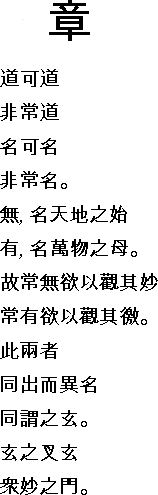
\includegraphics[width=0.30\textwidth]{tao.png}
\end{wrapfigure}

\noindent
\vspace{-10pt}
\begin{flushright}
The "Tao" is too great to be described by the name "Tao".
If it could be named so simply, it would not be the eternal Tao.\vspace{10pt}\linebreak
Heaven and Earth began from the nameless (Tao),
but the multitudes of things around us were created by names.\vspace{10pt}\linebreak
We desire to understand the world by giving names to the things we see, but these things are only the effects of something subtle.\vspace{10pt}\linebreak
When we see beyond the desire to use names, we can sense the nameless cause of these effects. \vspace{10pt}\linebreak
The cause and the effects are aspects of the same, one thing.
They are both mysterious and profound.\vspace{20pt}\linebreak
At their most mysterious and profound point lies the \textit{"Gate of the Great Truth"}.
\end{flushright}

\epigraph{People must have righteous principles in the first, and then they will not fail to perform virtuous actions.}{\textit{\footnotesize{Martin Luther}}}

\section{Principles}

Principles are the extensions of philosophies that derive frameworks of thought and act as guidelines of proper conduct between ourselves and others.

\subsection{Individual}

\begin{enumerate}
\item \textbf{Evaluate} as a means to greater \textbf{Knowledge}
\item \textbf{Happiness} as a result of \textbf{Virtue}
\item \textbf{Respect} as a result of \textbf{Depth}
\item \textbf{Freedom} as the truest \textbf{Expression}
\end{enumerate}

\subsection{Collective}

\begin{enumerate}
\item \textbf{Objective} with Receptivity, \textbf{Honest} with Communication
\item \textbf{Respectful} in Conduct, \textbf{Understanding} in Conflict
\item \textbf{Honor} to spoken Word, \textbf{Harmony} to Action
\end{enumerate}

\section{How We Make Change}

The cells of our body work together to provide the capacity for life. Similarly, we can compare the cells of our planet to each individual. 
If we understand the benefits of cooperation, challenges can be resolved thoroughly and quickly without unnecessary difficulties.
This is how we make change; we work together to resolve challenges with viable solutions.
This is the most efficient and effective way to bring change in the direction of our greatest preferences.\\

\noindent The community is the very foundation of an economy. An economy is only as strong as its foundation. 
When people loose faith in an economy, the base of the economy will collapse and the value of its system will fall with it. 
The Nexus community is already very resilient to the stress of markets. The community is a positive and inclusive group of people from across the world who are all aiming towards the same goals of transparency, prosperity, and freedom.\\ 

\noindent Nexus aims to build a strong community based on a savings culture and charity. 
The savings culture has been long lost but it is the best insurance policy for any uncertain times that may lie ahead. 
This helps the community hedge itself against high risk and volatile markets.
The idea is that your community member is your neighbor. If your neighbor does well, your local economy will prosper as well. 

\section{List of Contributors}

\begingroup
\parindent 0pt
\parskip  8pt

\begin{enumerate}
\item 
\printcontributor{Cantrell}

\item
\printcontributor{Reeg}

\item
\printcontributor{Gmyrek}

\item
\printcontributor{pSmith}

\item
\printcontributor{kSmith}

\item
\printcontributor{jSmith}

\item
\printcontributor{Mara}

\item
\printcontributor{Nexus}
\end{enumerate}

\endgroup

\pagebreak
\begin{thebibliography}{7}

\bibitem{bitcoin}
Bitcoin: A Peer-to-Peer Electronic Cash System \url{https://bitcoin.org/bitcoin.pdf}

\bibitem{hyperinflation}
What are some historic examples of hyperinflation? Investopedia.
\url{http://www.investopedia.com/ask/answers/061515/what-are-some-historic-examples-hyperinflation.asp}

\bibitem{cbc}
William F. Ehrsam, Carl H. W. Meyer, John L. Smith, Walter L. Tuchman, "Message verification and transmission error detection by block chaining", US Patent 4074066, 1976 \url{https://en.wikipedia.org/wiki/Block_cipher_mode_of_operation}

\bibitem{meshnetworks}
Mesh networking. Wikipedia.
\url{https://en.wikipedia.org/wiki/Mesh_networking}

\bibitem{githubnexusreleases}
Nexus releases on GitHub.com
\url{https://github.com/Nexusoft/Nexus/releases}

\bibitem{skminer}
SKMiner
\url{https://github.com/BitSlapper/SKMiner}

\bibitem{wolfniro}
Wolf Niro Miner
\url{https://github.com/OhGodAPet/Wolf-Niro-Miner}

\bibitem{wikiclockdrift}
Clock Drift. Wikipedia.
\url{https://en.wikipedia.org/wiki/Clock_drift}

\bibitem{nexusearth}
NexusEarth.com
\url{http://nexusearth.com/}

\bibitem{wikihash}
Cryptographic hash function. (2016, December 1). Wikipedia, The Free Encyclopedia. Retrieved 01:37, May 18, 2017 from \url{https://simple.wikipedia.org/w/index.php?title=Cryptographic_hash_function&oldid=5540578.}

\bibitem{peercoin}
King, S.; Nadal, S. (August 12, 2012). "PPCoin: Peer-to-peer crypto-currency with proof-of-stake" (PDF). peercoin.net. Retrieved 2013-12-23. \url{https://peercoin.net/assets/paper/peercoin-paper.pdf}

\bibitem{sect571r1} 
SEC 2: Recommended Elliptic Curve Domain Parameters, Daniel R. L. Brown (dbrown@certicom.com), Version 2.0, Section 3.7.2. 2010. Retrieved Jan 27, 2017 \url{http://www.secg.org/sec2-v2.pdf}

\bibitem{secp256k1}
secp256k1. Bitcoin Wiki.
\url{https://en.bitcoin.it/wiki/Secp256k1}

\bibitem{NIST_POST_QUANTUM}
Submission Requirements for Post Quantum Cryptography
\url{https://csrc.nist.gov/csrc/media/projects/post-quantum-cryptography/documents/call-for-proposals-final-dec-2016.pdf}
 
\bibitem{sha256bitcoin} 
Block hashing algorithm, Bitcoin Wiki \url{https://en.bitcoin.it/wiki/Block_hashing_algorithm}

\bibitem{wikisha2}
SHA-2. Wikipedia.
\url{https://en.wikipedia.org/wiki/SHA-2}

\bibitem{skeinpaper}
The Skein Hash Function Family. Version 1.3 — 1 Oct 2010.
\url{http://www.skein-hash.info/sites/default/files/skein1.3.pdf}

\bibitem{sha3announce} 
NIST Releases SHA-3 Cryptographic Hash Standard \url{https://www.nist.gov/news-events/news/2015/08/nist-releases-sha-3-cryptographic-hash-standard}

\bibitem{hashcash}
Hashcash - A Denial-of-Service Countermeasure. Adam Back. 2002. \url{http://www.hashcash.org/hashcash.pdf}

\bibitem{googlesha1}
Google Security Blog: Announcing the First SHA1 Collison. Feb 23, 2017.
\url{https://security.googleblog.com/2017/02/announcing-first-sha1-collision.html}

\bibitem{nistcompetitionend}
NIST: SHA-3 Winner, October 2nd, 2010
\url{http://csrc.nist.gov/groups/ST/hash/sha-3/winner_sha-3.html}

\bibitem{nobelfeynman}
The Nobel Prize in Physics 1965 was awarded jointly to Sin-Itiro Tomonaga, Julian Schwinger and Richard P. Feynman "for their fundamental work in quantum electrodynamics, with deep-ploughing consequences for the physics of elementary particles"
\url{http://www.nobelprize.org/nobel_prizes/physics/laureates/1965/}

\bibitem{grover2qubits}

Nature: FIGURE 4. Implementation of Grover's search algorithm, July 9th, 2009
\url{http://www.nature.com/nature/journal/v460/n7252/fig_tab/nature08121_F4.html}

\bibitem{groversalgorithm}

Estimating Cost of generic quantum pre-image attacks, October 13th, 2016
\url{https://arxiv.org/pdf/1603.09383.pdf}

\bibitem{cdhalving}
Will Bitcoin's Block Rewards Halving Bring Crisis or Consistency? CoinDesk.
\url{http://www.coindesk.com/crisis-halving-bitcoin-mining/ip}

\bibitem{quantumattacks}

Quantum Attacks on Public Key Cryptosystems, Song Y. Yan 2013

\url{http://www.springer.com/us/book/9781441977212}

\bibitem{bitcorepkh}
bitcore-lib docs. Script section.
\url{https://github.com/bitpay/bitcore-lib/blob/master/docs/script.md}

\bibitem{goldenmean}
Golden Mean.
\url{http://www.anus.com/zine/articles/draugdur/golden_mean/}

\bibitem{n_ethics}
Nicomachean Ethics. Wikipedia.
\url{https://en.wikipedia.org/wiki/Nicomachean_Ethics}

\bibitem{aynrand}
Objectivism (Ayn Rand). Wikipedia.
\url{https://en.wikipedia.org/wiki/Objectivism_(Ayn_Rand)}

\bibitem{kingdomofends}
Kingdom of Ends. Wikipedia.
\url{https://en.wikipedia.org/wiki/Kingdom_of_Ends}

\bibitem{aristotle}
Aristotole. Wikipedia.
\url{https://en.wikipedia.org/wiki/Aristotle}

\bibitem{kant}
Immanuel Kant. Wikipedia.
\url{https://en.wikipedia.org/wiki/Immanuel_Kant}

\bibitem{tao_introduction}
TheTao.info
\url{http://www.thetao.info/index.htm}

\bibitem{tao_chapter1}
TheTao.info Chaper 1.
\url{http://www.thetao.info/english/page1.htm}

\bibitem{tragedycommons}
Tragedy of the Commons. Investopedia.
\url{http://www.investopedia.com/terms/t/tragedy-of-the-commons.asp}

\bibitem{primesolominer}
Nexus Prime Solo Miner Source Code, Github.com
\url{https://github.com/Nexusoft/PrimeSoloMiner}

\bibitem{nxsprimecom}
NXSPrime.com
\url{http://nxsprime.com}

\bibitem{wikiprobable}
Probable prime. Wikipedia.
\url{https://en.wikipedia.org/wiki/Probable_prime}

\bibitem{wikifermat}
Fermat primality test. Wikipedia.
\url{https://en.wikipedia.org/wiki/Fermat_primality_test}

\bibitem{findingprimeclusterspaper}
Finding Clusters of Primes, I, Jorg Waldvogel and Peter Leikauf, January 2003.
\url{http://www.sam.math.ethz.ch/~waldvoge/Projects/clprimes03.pdf}

\bibitem{wolframprimecluster}
Prime Constellation - Wolfram MathWorld
\url{http://mathworld.wolfram.com/PrimeConstellation.html}

\bibitem{wikiprimecluster}
Wikipedia. Prime k-tuple: Prime Constellations
\url{https://en.wikipedia.org/wiki/Prime_k-tuple#Prime_constellations}

\bibitem{physicsmathprime}
Quantum Magazine: Physicists Attack Math's \$1,000,000 Question.
\url{https://www.quantamagazine.org/quantum-physicists-attack-the-riemann-hypothesis-20170404/}

\bibitem{shorarxiv}
Polynomial-Time Algorithms for Prime Factorization and Discrete Logarithms on a Quantum Computer. Peter W. Shor (AT\&T Research).
\url{http://arxiv.org/abs/quant-ph/9508027}

\bibitem{prooszalka}
J. Proos, C. Zalka, Shor's discrete logarithm quantum algorithm for elliptic curves. Quant. Inf. Comput. 3(4), 317-344 (2003).
\url{https://arxiv.org/abs/quant-ph/0301141}

\bibitem{kayezalka}
Optimized quantum implementation of elliptic curve arithmetic over binary fields. Phillip Kaye, Christof Zalka. 2004.
\url{https://arxiv.org/abs/quant-ph/0407095}

\bibitem{registersha3}
SHA3-256 is quantum-proof, should last BEELLIONS of years, say boffins. The Register.
\url{http://www.theregister.co.uk/2016/10/18/sha3256_good_for_beelions_of_years_say_boffins/}

\bibitem{cryptosha3}
Estimating the cost of generic quantum pre-image attacks on SHA-2 and SHA-3
\url{http://eprint.iacr.org/2016/992}

\bibitem{sigleak}
"Ooh Aah... Just a Little Bit" : A small amount of side channel can go a long way. N. Benger, J. van der Pol, Nigel P. Smart and Y. Yarom.
\url{http://eprint.iacr.org/2014/161}

\bibitem{sidechannel}
Recovering OpenSSL ECDSA Nonces Using the FLUSH+RELOAD Cache Side-channel Attack. Yuval Yarom. Naomi Benger. February 24, 2014.
\url{https://eprint.iacr.org/2014/140.pdf}

\bibitem{weusesand}
The Amazing Math of Bitcoin Private Keys - James DeAngelo. WeUseCoins.com.
\url{https://www.weusecoins.com/amazing-math-bitcoin-private-keys/}

\bibitem{bitwiki256}
SHA-256. Bitcoin Wiki.
\url{https://en.bitcoin.it/wiki/SHA-256}

\bibitem{sha3}
SHA-3. Wikipedia.
\url{https://en.wikipedia.org/wiki/SHA-3}

\bibitem{nistgovk}
NIST Selects Winner of Secure Hash Algorithm (SHA-3) Competition. October 02, 2012. NIST.gov
\url{https://www.nist.gov/news-events/news/2012/10/nist-selects-winner-secure-hash-algorithm-sha-3-competition}

\bibitem{wikiskein}
Skein (hash function). Wikipedia.
\url{https://en.wikipedia.org/wiki/Skein_(hash_function)}

\bibitem{largebitcoin}
The Large Bitcoin Collider Is Generating Trillions of Keys and Breaking Into Wallets. Jordan Pearson. Apr 13 2017. MOTHERBOARD.
\url{https://motherboard.vice.com/en_us/article/nzpv8m/the-large-bitcoin-collider-is-generating-trillions-of-keys-and-breaking-into-wallets}

\bibitem{wikikeysize}
Key Size. Wikipedia.
\url{https://en.wikipedia.org/wiki/Key_size}

\bibitem{nsa384}
"Information Assurance". Nsa.gov. 2016-05-04. Archived on 2009-02-07. Retrieved July 2017.
\url{https://web.archive.org/web/20090207005135/http://www.nsa.gov/ia/programs/suiteb_cryptography/index.shtml}

\bibitem{bruteforce}
Cryptography/Brute force attack. Wikibooks.org. Retrived on July 2, 2017.
\url{https://en.wikibooks.org/wiki/Cryptography/Brute_force_attack}

\bibitem{p2pkh}
Bitcoin Developer Guide. P2PKH Script Validation. Bitcoin.org
\url{https://bitcoin.org/en/developer-guide#p2pkh-script-validation}

\bibitem{lovgrover}
A fast quantum mechanical algorithm for database search. Lov K. Grover (Bell Labs, Murray Hill NJ)
\url{https://arxiv.org/abs/quant-ph/9605043}

\end{thebibliography}

\end{document}